\documentclass[A4,12PT, english, twocolumn]{journal}
\usepackage{amsmath,amssymb,amsfonts}
\usepackage[margin=0.7in]{geometry}
\usepackage{graphicx}
\usepackage{enumitem}
\usepackage{xcolor}
\usepackage{hyperref}
\usepackage{tabularray}
\usepackage{multicol}
\usepackage{tikz}
\usepackage{circuitikz}
\usepackage{scalerel}
\usepackage{pict2e}
\usepackage{tkz-euclide}
\usetikzlibrary{calc}
\usetikzlibrary{patterns,arrows.meta}
\usetikzlibrary{shadows}
\usetikzlibrary{external}

%pgfplots
\usepackage{pgfplots}
\pgfplotsset{compat=newest}
\usepgfplotslibrary{statistics}
\usepgfplotslibrary{fillbetween}

\def\infinity{\rotatebox{90}{8}}

% Hiperlink
\hypersetup{
    colorlinks=true,
    linkcolor=blue,
    filecolor=magenta,      
    urlcolor=cyan,
    pdftitle={Overleaf Example},
    pdfpagemode=FullScreen,
}
%\usepackage{style}
\NewDocumentCommand{\Log}{o}{%
\IfNoValueTF{#1}{}{{}^{#1}\!}\log}%
  
%command buat logaritma dengan basisnya di pojok kiri
%\textheight=17cm
%\textwidth=10cm
%\usepackage{blindtext}
\setenumerate[1]{itemsep=0,5cm}
\setenumerate[2]{topsep=5pt, itemsep=5pt, label=\textbf{\Alph*}.}

\title{Matematika Saintek \& Fisika UTUL UGM 2018 Kode 276}
\author{Fauzan Akbar Sukandar Putra \\ \LaTeX}

\begin{document}

\maketitle

%\begin{minipage}{0.5\textwidth}
\begin{enumerate}
%1%
\item Diberikan segitiga sama kaki dengan panjang alasnya $10 \; cm$ dan tingginya $6 \; cm$. Di dalam segitiga ini dibuat persegi panjang dengan salah satu sisinya terletak pada alas segitiga tersebut. Luas maksimum persegi panjang tersebut adalah \dots
    \begin{enumerate}
        \item $10 \; cm^2$
        \item $12 \; cm^2$
        \item $15 \; cm^2$
        \item $18 \; cm^2$
        \item $20 \; cm^2$
    \end{enumerate}
  
%2%
\item $\lim\limits_{x \longrightarrow \frac{\pi}{2}}{\left(\pi - 2x \right)\tan x =}$ \dots
    \begin{enumerate}
        \item $1$
        \item $2$
        \item $-1$
        \item $-2$
        \item $0$
    \end{enumerate}
     
%3%
\item Salah satu akar dari persamaan $x^3+ax^2+bx+c=0$ adalah $0$ sedangkan dua akar lainnya saling berlawanan tanda. Jika $a+b+c=-4$, maka akar terbesar yang mungkin adalah \dots
    \begin{enumerate}
        \item $2$
        \item $4$
        \item $8$
        \item $16$
        \item $32$
    \end{enumerate}
   
%4%
\item Himpunan penyelesaian pertidaksamaan \\ $\left|x-5 \right|^2-3 \left|x-5 \right| + 2 < 0$ adalah \dots
    \begin{enumerate}
        \item $\left(3,4 \right) \cup \left[6,7 \right)$
        \item $\left(3,4 \right) \cup \left(6,7 \right)$
        \item $\left(1,2 \right) \cup \left(3,4 \right]$
        \item $\left(- \infinity,1 \right) \cup \left[6, \infinity \right)$
        \item $\left(- \infinity,2 \right) \cup \left(3,7 \right)$
    \end{enumerate}

%5%
\item Jika $m$ adalah bilangan real sedemikian sehingga sistem persamaan
\begin{center}
    \begin{cases}
        5x-7y=mx \\
        2x-3y=my \\
    \end{cases}
\end{center}
mempunyai solusi $\left(x,y \right)$ yang tidak keduanya nol. Maka $m^2-2m=$ \dots
    \begin{enumerate}
        \item $-2$
        \item $-1$
        \item $0$
        \item $1$
        \item $2$
    \end{enumerate}
    
%6%  
\item Misalkan $A$ dan $B$ adalah sudut-sudut lancip sehingga $\sin{A} = \frac{1}{\sqrt{5}}$ dan $\cos{B} = \frac{3}{\sqrt{10}}$. Besar sudut $\left(A+B \right)$ \\ adalah \dots
    \begin{enumerate}
        \item $\frac{\pi}{6}$
        \item $\frac{\pi}{4}$
        \item $\frac{\pi}{3}$
        \item $\frac{\pi}{6}$
        \item $\pi$
    \end{enumerate}
    
%7%
\item Diberikan persamaan
\begin{center}
    $2\sin^3{x} - \cos^2{x} - 2\sin{x} = 0$. \; $0 \leq x \leq \frac{3\pi}{2}$.
\end{center}
Jika $x_1$ penyelesaian terkecil dan $x_2$ penyelesaian terbesar dari persamaan tersebut, maka $x_2-x_1=$ \dots
    \begin{enumerate}
        \item $\frac{\pi}{3}$
        \item $\frac{2\pi}{3}$
        \item $\pi$
        \item $\frac{4\pi}{3}$
        \item $\frac{5\pi}{3}$
    \end{enumerate}
    
%8%  
\item Akar-akar persamaan $x^3-7x^2+px+q=0$ membentuk deret geometri dengan rasio $2$. Nilai $p+q$ adalah \dots
    \begin{enumerate}
        \item $2$
        \item $4$
        \item $6$
        \item $12$
        \item $14$
    \end{enumerate}
    
%9%
\item Jika $2 \; \cdot \; ^4\Log x - ^4\Log {\left(4x+3 \right)} = -1$, maka $^2\Log x =$ \dots
	\begin{enumerate}
		\item $^2\Log {3} - 1$
		\item $^2\Log {3} + 1$
		\item $1 - \; ^2\Log {3}$
		\item $-1 - \; ^2\Log {3}$
		\item $^2\Log {3} + \; ^3\Log {2}$
	\end{enumerate}
	
%10%
\item Jika $\alpha$ dan $\beta$ adalah akar dari persamaan
\begin{center}
    $^x\Log{3} - \; ^x\Log{\left(2x-4+ \frac{4}{x} \right)} = 1$.
\end{center}
Maka $\alpha + \beta =$ \dots
   \begin{enumerate}
        \item $-2$
        \item $-1$
        \item $0$
        \item $2$
        \item $4$
   \end{enumerate}
   
%11%
\item Diberikan garis $y= \frac{x}{3}$ dan $y=3x$. Persamaan lingkaran yang menyinggung dua garis tersebut, berpusat di $\left(-a,-a \right). \; a>0$. dan berjari-jari $\frac{6}{\sqrt{10}}$ adalah \dots
    \begin{enumerate}
        \item $x^2+y^2+6x+6y+\frac{72}{5}=0$
        \item $x^2+y^2+6x+6y+\frac{82}{5}=0$
        \item $x^2+y^2+8x+8y+\frac{72}{5}=0$
        \item $x^2+y^2+9x+9y+\frac{62}{5}=0$
        \item $x^2+y^2+9x+9y+\frac{82}{5}=0$
    \end{enumerate}
  
%12%  
\item Fungsi $f \left(x \right) = - \cos{2x} + \sqrt{3}\sin{2x} + 1, \; 0 \leq x \leq \pi$. mencapai ekstrim pada saat $x=x_1$ dan $x=x_2$. Nilai $x_1+x_2$ adalah \dots
    \begin{enumerate}
        \item $\frac{\pi}{3}$
        \item $\frac{2\pi}{3}$
        \item $\frac{7\pi}{6}$
        \item $\frac{4\pi}{3}$
        \item $\frac{5\pi}{3}$
    \end{enumerate}
    
%13% 
\item Diberikan vektor $\Vec{u} = \left(a,b,c \right)$ dan $
\Vec{v} = \left(b,a,3 \right)$. juka \\ $\Vec{u} \cdot \Vec{v} = \left| {\left| \Vec{u} \right|} \right|^2$ dan $\left| {\left| \Vec{u} - \Vec{v} \right|} \right|^2 = 5$. Maka nilai $c^3+2c+2$ yang mungkin adalah \dots
    \begin{enumerate}
        \item $-2$
        \item $-1$
        \item $2$
        \item $5$
        \item $14$
    \end{enumerate}

%14%
\item Invers dari matriks $A$ adalah
\begin{center}
    \begin{pmatrix}
        \frac{1}{a-b} & \frac{1}{a+b}\\
        \frac{-1}{a-b} & \frac{1}{a+b}
    \end{pmatrix}
\end{center}
Jika $B=2A$, maka matriks $B$ adalah \dots
\begin{enumerate}
       \item    \begin{pmatrix}
                    a-b & a-b\\
                    a+b & a+b
                \end{pmatrix}
        \item   \begin{pmatrix}
                    a-b & -a+b\\
                    a+b & a+b
                \end{pmatrix}
        \item   \begin{pmatrix}
                    a-b & -a+b\\
                    -a-b & a+b
                \end{pmatrix}
        \item   \begin{pmatrix}
                    -a+b & a-b\\
                    a+b & a+b
                \end{pmatrix}
        \item   \begin{pmatrix}
                    a+b & a-b\\
                    a+b & -a+b
                \end{pmatrix}
    \end{enumerate}

%15% 
\item Diberikan $ABC$ segitiga sama kaki dengan $AB=AC$ dan $\angle BAC= \alpha$. Misalkan titik $D$ pada sisi $BC$ sehingga $AD$ garis tinggi. Jika $BC=2$ dan $AD=1$, \\ maka $\sin \angle BAC =$ \dots
    \begin{enumerate}
        \item $\frac{1}{\sqrt{2}}$
        \item $\frac{1}{2}$
        \item $\frac{2}{\sqrt{2}}$
        \item $2$
        \item $1$
    \end{enumerate}
    

%FISIKA %
%16%
\newpage
\item Sebuah balok bermassa $m$ mula-mula bergerak ke kanan pada suatu permukaan horizontal licin dengan kecepatan $v$. Balok tersebut kemudian menekan pegas dengan konstanta pegas $k$. Ketika energi kinetik balok sama dengan energi potensial pegas, besarnya jarak yang ditempuh balok saat menekan pegas adalah \dots
    \begin{enumerate}
        \item $v \sqrt{\frac{m}{2k}}$
        \item $v \sqrt{\frac{m}{k}}$
        \item $v \sqrt{\frac{2m}{k}}$
        \item $2v \sqrt{\frac{m}{k}}$
        \item $\frac{1}{2} v \sqrt{\frac{m}{k}}$
    \end{enumerate}
  
%17%
\item Sebuah peluru bermassa $2 \; kg$ yang ditembakkan dari tanah dengan sudut elevasi dan kecepatan awal tertentu memiliki ketinggian maksimum dan jangkauan maksimum berturut-turut $25 \; m$ dan $40 \; m$. Energi kinetik peluru pada saat ditembakkan adalah \dots
    \begin{enumerate}
        \item $500 \; J$
        \item $580 \; J$
        \item $625 \; J$
        \item $800 \; J$
        \item $1000 \; J$
    \end{enumerate}
     
%18%
\item Tekanan total di dalam suatu fluida pada kedalaman $h_1$ adalah $P_1$. Sedangkan pada kedalaman $h_2$, tekanan totalnya adalah $P_2$. Jika tekanan atmosfer adalah $=P_0$, maka tekanan total pada kedalaman $h_1+h_2$ adalah \dots
    \begin{enumerate}
        \item $P_1+P_2$
        \item $P_1+P_2-P_0$
        \item $P_1+P_2+P_0$
        \item $P_1+P_2-2P_0$
        \item $P_1+P_2+2P_0$
    \end{enumerate}
   
%19%
\item Sebuah pegas ringan memiliki tetapan pegas $500 \; N/m$. Salah satu ujung pegas itu diikat pada balok yang terletak di lantai yang cukup licin, sedangkan ujung yang lain ditarik (lihat gambar) dengan gaya yang tetap sehingga balok mengalami percepatan $5 \, m/s^2$ dan pegas bertambah panjang $1 \; cm$. Jika diatas balok itu deletakkan sebuah balok lain yang bermassa sama sehingga percepatannya menjadi $2,5 \; m/s^2$, berapakah pertambahan panjang pegas sekarang? \dots
\begin{center}
    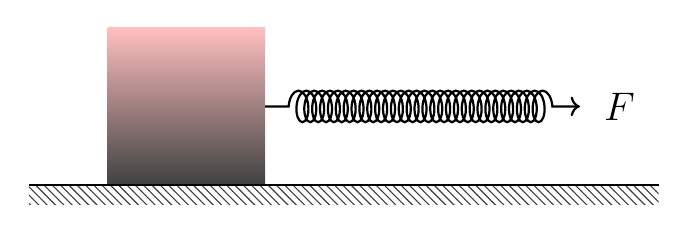
\begin{tikzpicture}
        %GRID
        %\draw[lightgray] (0,0) grid (5,5);

        %PEGAS
        \draw
        [
            thick, ->,
            decoration={
                coil,
                segment length = 1mm,
                amplitude = 2mm,
                aspect = 0.5,
                post length = 3mm,
                pre length = 3mm},
            decorate] (2,1) -- (6,1) node[right=5pt]{\Large $F$};
        
        %BALOK
        \shade[top color=pink, bottom color=darkgray] (0,0) rectangle (2,2);

        %LANTAI
        \fill[pattern=north west lines, pattern color=darkgray] (-1,-0.25) rectangle (7,0);
        \draw[thick] (-1,0) -- (7,0);
    \end{tikzpicture}
\end{center}
    \begin{enumerate}
        \item $1,0 \; cm$
        \item $2,0 \; cm$
        \item $2,4 \; cm$
        \item $2,8 \; cm$
        \item $3,2 \; cm$
    \end{enumerate}

%20%
\item Sebuah elektron bergerak ke kanan horizontal memasuki suatu wilayah dengan medan magnet seragam mengarah ke atas. Gaya yang dialami elektron saat memasuki wilayah tersebut adalah mengarah \dots
    \begin{enumerate}
        \item Ke atas 
        \item Ke bawah 
        \item Ke luar bidang gambar 
        \item Masuk bidang gambar 
        \item Ke kiri
    \end{enumerate}

%21%
\item Sebuah induktor dengan induktansi $10 \; mH$, sebuah resistor, dan baterai ideal dipasangkan dalam rangkaian secara serial. Ketika arus dalam rangkaian adalah $1 \, A$, maka besar energi yang tersimpan dalam induktor adalah \dots
    \begin{enumerate}
        \item $5 \; mJ$
        \item $15 \; mJ$
        \item $20 \; mJ$
        \item $25 \; mJ$
        \item $50 \; mJ$
    \end{enumerate}
    
%22% 
\item Sebuah kawat tak hingga panjang beraliran arus listrik $I_0$. Sebuah elektron dilepaskan pada jarak $a$ dari kawat dengan kecepatan awal $v_0$ menjauhi kawat. Setelah beberapa saat arah gerak elektron mmenuju kawat, kecepatan elektron ketika itu adalah \dots
    \begin{enumerate}
        \item $v_0$
        \item $2v_0$
        \item $v_0 \; ln \; 3$
        \item $\frac{v_0}{2}$
        \item $v_0 \; ln \; 2$
    \end{enumerate}
    
%23%
\item Sebuah pegas dengan  konstanta pegas $k$ dipakai untuk menggantungkan suatu benda bermassa $m$. Sistem benda pegas ini kemudian diosilasikan dan berosilasi dengan periode $T$. Pegas kemudian dipotong menjadi tiga dan ketiganya dipasangkan ke benda lain secara paralel. Ketika benda kedua diosilasikan, periode osilasinya juga $T$. Maka massa benda kedua adalah \dots
    \begin{enumerate}
        \item $3 \; m$
        \item $6 \; m$
        \item $9 \; m$
        \item $12 \; m$
        \item $15 \; m$
    \end{enumerate}
    
%24%
\item Gelombang bunyi dengan frekuensi $256 \; Hz$ merambat di udara dengan kecepatan $330 \; m/s$. Cepat rambat gelombang bunyi dengan frekuensi $512 \; Hz$ di udara adalah \dots
	\begin{enumerate}
		\item $82,5 \; m/s$
		\item $165 \; m/s$
		\item $330 \; m/s$
		\item $347,5 \; m/s$
		\item $660 \; m/s$
	\end{enumerate}
	
%25%
\item Pada suatu pola difraksi celah tunggal dengan lebar celah $a$, terdapat difraksi minimum pertama pada sudut $x^\ciirc$. Bila celah tunggal tadi diganti dengan celah ganda berjarak $d$, maka posisi gelap pertama tidak akan berubah bila \dots
   \begin{enumerate}
        \item $d=a$
        \item $d= \frac{a}{2}$
        \item $d= \frac{a}{\sqrt{2}}$
        \item $d= \frac{a}{3}$
        \item $d= \frac{a}{\sqrt{3}}$
   \end{enumerate}
   
%26%
\item Sebuah benda yang diletakkan $10 \; cm$ dari cermin cekung menghasilkan bayangan nyata berjarak $8 \; cm $ dari cermin. Jika benda tersebut dipindahkan ke posisi baru sejauh $40 \; cm$ dari cermin, maka posisi bayangan dan sifatnya adalah \dots 
    \begin{enumerate}
        \item $3,5 \; cm$ di depan cermin, nyata
        \item $4,2 \; cm$ di belakang cermin, maya
        \item $5,0 \; cm$ di depan cermin, nyata
        \item $6,4 \; cm$ di belakang cermin, maya
        \item $7,5 \; cm$ di depan cermin, nyata
    \end{enumerate}
  
%27%
\item Dua lensa cembung masing-masing dengan fokus sebesar $15 \; cm$ diletakkan terpisah sejauh $40 \; cm$. Jika suatu benda diletakkan $30 \; cm$ dari lensa pertama, maka bayangan terakhir yang terbentuk akan memiliki pembesaran total sebesar \dots
    \begin{enumerate}
        \item $2$ kali
        \item $3$ kali
        \item $4$ kali
        \item $5$ kali
        \item $6$ kali
    \end{enumerate}
    
%28% 
\item Suatu gas ideal mengalami proses ekspansi. Selama ekspansi energi dalamnya tidak berubah. Bila awalnya tekanannya adalah $1 \times 10^5 \; Pa$ dan volumenya $1 \; m^3$, maka berikut ini adalah nilai tekanan dan volume yang mungkin bagi gas ideal tadi \dots
    \begin{enumerate}
        \item $P=1 \times 10^5 \; Pa$, $V=2m^3$
        \item $P=2 \times 10^5 \; Pa$, $V=1m^3$
        \item $P=2 \times 10^5 \; Pa$, $V=3m^3$
        \item $P=0,5 \times 10^5 \; Pa$, $V=2m^3$
        \item $P=0,1 \times 10^5 \; Pa$, $V=3m^3$
    \end{enumerate}

%29%
\item Pada saat air membeku termometer $X$ menunjukkan angka $-10^\circ \; X$ dan pada saat mendidih menunjukkan angka $140^\circ \; X$. Jika termometer Celcius menunjukkan angka $30^\circ \; C$, maka termometer $X$ menunjukkan angka \dots
    \begin{enumerate}
        \item $30^\circ \; X$
        \item $35^\circ \; X$
        \item $37,5^\circ \; X$
        \item $40^\circ \; X$
        \item $45^\circ \; X$
    \end{enumerate}

%30%
\item Pada atom Hidrogen besar jari-jari kulit elektron nomor $n$ dan momentum sudutnya berturut-turut adalah $r_n$ dan $L_n$ dengan konstanta positif $C$ adalah \dots
    \begin{enumerate}
        \item $\frac{L_n^2}{r_n}=C$
        \item $\frac{L_n}{r_n}=C$
        \item $L_n r_n=C$
        \item $\frac{r_n^2}{L_n}=C$
        \item $L_n^2 r_n=C$
    \end{enumerate}
 
%31%
\item Suatu partikel bergerak dengan kecepatan $0,4 \; c$ sepanjang sumbu $x$ pada kerangaka $S'$. Jika kerangka $S'$ bergerak dengan kecepatan $0,6 \; c$ terhadap kerangka $S$ searah dengan arah kecepatan partikel, maka kecepatan partikel relatif terhadap kerangka $S$ adalah sebesar \dots
    \begin{enumerate}
        \item $0,2 \; c$
        \item $0,4 \; c$
        \item $0,6 \; c$
        \item $0,8 \; c$
        \item $1,0 \; c$
    \end{enumerate}

%32%
\item Sebuah partikel bermassa $m$ dan bermuatan $+q$ dipercepat dari keadaan diam menuju beda potensial $V$ kemudian memasuki medan magnet seragam $B$ yang arahnya tegak lurus kecepatan partikel. Jari-jari lintasan partikel adalah \dots
    \begin{enumerate}
        \item $\sqrt{\frac{2mV}{qB}}$
        \item $\sqrt{\frac{mV}{qB^2}}$
        \item $\sqrt{\frac{mV}{qB}}$
        \item $\sqrt{\frac{mV}{2qB^2}}$
        \item $\sqrt{\frac{2mV}{qB^2}}$
    \end{enumerate}

%33%
\item Suatu benda hitam pada suhu $T \, (K)$ memancarkan energi $E$. Jika dinaikkan suhunya sebesar $200^\circ \; C$, energinya adalah $16E$. Jika kemudian dinaikkan lagi sebesar $200^\circ \; C$, energinya adalah $nE$. Nilai $n$ adalah \dots
    \begin{enumerate}
        \item $32$
        \item $81$
        \item $256$
        \item $324$
        \item $1024$
    \end{enumerate}

%34%
\item Suatu partikel relativistik memiliki  energi diam $E_0$ momentum $p$ dan energi $K$. Misalnya $\frac{pc}{E_0}=x$, maka $\frac{K}{E_0}=$ \dots
    \begin{enumerate}
        \item $-1+ \sqrt{1+x^2}$
        \item $-1+ \sqrt{1-x^2}$
        \item $1- \sqrt{x^2-1}$
        \item $1- \sqrt{1-x^2}$
        \item $1+ \sqrt{1-x^2}$
    \end{enumerate}

%35%
\item Bila diketahui jarak bumi dan bulan adalah $380.000 \; km$ dan jari-jari bumi adalah $6400 \; km$, maka kecepatan minimum yang dibutuhkan bulan untuk dapat lepas dari pengaruh gravitasi bumi adalah \dots $m/s$
    \begin{enumerate}
        \item $1453$
        \item $145,3$
        \item $14,53$
        \item $1,453$
        \item $0,1453$
    \end{enumerate}

\end{enumerate}
\end{document}  
